

\section{General MRI pre-processing}
Maybe do a top saying something about the program we choose to use. Derved lave en afgrænsning der 


There are multiple steps to preprocess fMR images depending on the apparent application and outcome intended. However, there is a standard set of methods that is usually used across all applications. The following section seek to elucidate some of the most commonly used correction methods, including those considered for the standard preprocessing method used in this project. An example of some of the general processing steps for MR imaging can be seen on \figref{fig:back:pipeline}.\cite{Poldrack2011} 

\begin{figure}[H]                 
	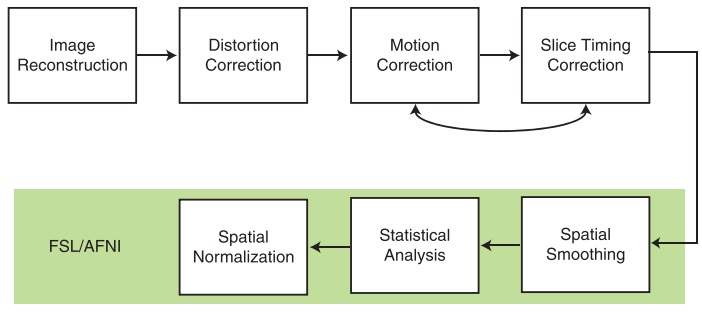
\includegraphics[width=.8\textwidth]{figures/aBackground/processing}  
	\caption{The general pipeline for MRI processing done in either FSL or AFNI, showing the different processing steps considered before final statistical analysis. Modified from \cite{Poldrack2011}.}
	\label{fig:back:pipeline} 
\end{figure}


\subsection{Quality control}
Conducting a continues quality control is highly recommended after each performed correction step. Various scanner artifacts can occur while acquiring an MRI series. Before performing any common correction steps, one should consider to look for spike or ghosting artifacts. Spike artifacts are seen as a regular pattern of change in brightness across the entire image. This problem can occur due to instability inside the scanner deriving from e.g. electrical discharges.  
The artifact called ghosting occur mainly due to two reasons. One being an offset in phase between different lines in K-space and the other due to periodic motion as in heartbeat and respiration. Ghosting can be seen as light copies of the object appearing to either side of the object. Both types of artifacts can corrupt the information contained in the images. However, artifacts of this kind rarely present themselves in newer scanners, nevertheless it is still recommended to perform a quality control of the scan.\cite{Poldrack2011}

\subsection{Distortion correction}

Some fMRI acquisition methods, including the most widely used method of gradient-echo echo planar imaging, suffers from artifacts at regions air and tissue meet. The ear canal and sinuses are areas especially vulnerable. Inhomogeneity in the magnetic field in these areas can cause two types of artifacts, dropout and geometric distortion. A dropout will result in a reduced signal intensity in regions close to the air to tissue transition. When a dropout during an acquisition occurs, the lost signal cannot be restored and the damage is permanent. Therefore it is wise to consider the appropriate acquisition method taking the area of interest into addition. Air to tissue passages can also be subject to spatial distortion due to inhomogeneity created in the magnetic field. This will lead to structures not being located correctly in the captured image. This distortion makes is difficult to align two different scans, as done when aligning fMRI images with structural images. 
The spatial distortion can partially be corrected by employing field maps. In order to do a field map, the pulse sequence from the scan needs to be known. The process involves acquiring images at two different echo times. This results in images with two different phases which can be used to compute the field inhomogeneity. Thereby it becomes possible to calculate the relative distance each voxel has shifted. This makes up a map for the distance shift for each voxel, and by inverting the map the original image can be restored.\cite{Poldrack2011}  

\subsection{Slice timing correction} 

Acquiring fMRI scans is nearly always done in two-dimensions, where the slices are taken one by one. This can either be in an ascending, descending or interleaved order. Interleaved order \fxnote{think it is done to avoid crosstalk} is sequentially skipping every either odd or even slice and then afterwards do to skipped slices. Regardless of which order the slices are acquired, a difference in effect in each slice to the same hemodynamic response will be present due to the time difference in the slices. The method and result of interleaved MRI acquisition order can be seen \figref{fig:back:interleaved} The difference in time between slices can range up to a couple of seconds depending on the acquisition protocol. 
\begin{figure}[H] 
	\subfigure[]
	{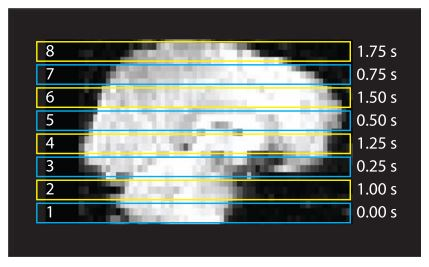
\includegraphics[width=.38\textwidth]{figures/aBackground/slice}} 
	\hspace{0.5cm}
	\subfigure[]
	{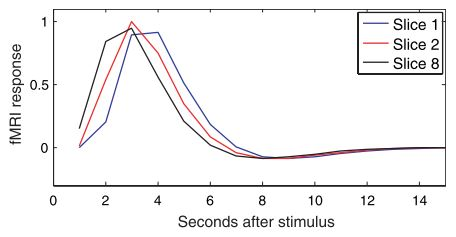
\includegraphics[width=.40\textwidth]{figures/aBackground/response}}  
	\hspace{0.5cm}
	\caption{Figure a illustrates an example of an MRI acquisition using interleaved order, where initially every odd slice is acquired followed by every even. The information about the hemodynamic response in each slice, and thereby also the difference at each time-point is shown in figure b. Figure modified from \cite{Poldrack2011}.}
	\label{fig:back:interleaved}
\end{figure}

The difference in slice timing constitutes a problem when analyzing the data. The data is formed into statistical model, but since this model assumes that all slices are acquired at the same time point, the actual signal and the statistical model creates a mismatch. To counter this problem slice timing correction was introduced. The common approach of this method is to choose a reference slice, usually the slice acquired at T/2, and use this slice to interpolate the others. Linear interpolation can be used for simplicity, but most often sinc interpolation is used as it imposes less smoothing to the signal.\cite{Poldrack2011} 

\subsection{Motion correction}

Correcting for motion artifacts when doing MRI is inevitable, since even the best subjects will not be able to hold still. Even subtle movements as swallowing will be visible in the raw acquired image.\cite{Poldrack2011} 

Multiple internal and external factors can cause a subject to move. Internal factors are none avoidable physiologic motion. The heartbeat causes a pulsating movement which makes the brain move. Additionally motion created during respiration can cause small changes in the magnetic field around the head. External factors like imposed stimulus might also cause the subject to make sudden movements. Often when doing fMRI the brain activation is measured while the subject is subjected to some kind stimulus. The stimulus would make the patient move, while some brain center might also show activation associated with stimulus,  and therefore it is easy to mistake brain activation with stimulus correlated movement when analyzing the data, resulting in a weaker or even false statistical analysis.\cite{Poldrack2011} 

Motion during image acquisition can result in two primary artifact effects, being bulk motion and spin history. Bulk motion refers to the movement of the head as a whole and requires standard correction methods, e.g. the images throughout the series to be realigned to a reference image. The effect of bulk motion can be visual in the entire image of the brain, but the effect will be most predominant at the edges of the brain. Here the artifact will be noticeable as either a drop or increase in intensity as a voxel would switch from containing brain tissue to suddenly not during head motion.  
Spin history is head movement interfering with MRI signal itself. The interference occur during acquisition when a voxel of excited protons is moved in to a neighboring slice. The scanner will thereby receive a different signal than expected which do not correctly represent the actual local properties. This results in an image where the intensities change in a striped pattern, visible when acquiring slices in interleaved order. The standard motion correction methods cannot cope with this type of artifact, but Independent Component Analysis (ICA) might be able to correct for this artifact.\cite{Poldrack2011} 

As mentioned earlier motion correction is to realign the series of images to a reference image trying to minimize cost in an introduced cost function. The reference image is usually the one taken midway into the series, justified by it being the closets to the average as well as the scanner at that time would have achieved stable contrast, as the magnetization would have reached steady state. The images are thereafter realigned utilizing an image registration method as it register the brain in each image. The general methods for motion correction treats the brain rigid objects, thus only performing rigid body transformations. Subsequently, the brain can either translate or rotate along the three axis, but the shape of the head cannot change. This method is therefore only applicable for bulk motion.\cite{Poldrack2011} 

\subsection{Spatial smoothing}

In some cases, introducing spatial smoothing in the preprocessing pipeline proves to be beneficial. Spatial smoothing allows the possibility of gaining a higher signal to noise ratio within the image, though with the consequence of a decrease in spatial resolution as the image gets blurred and smaller areas of activation gets smeared together. The operation can be justified by the closely neighboring pixel being correlated in effect to the hemodynamic response. Spatial smoothing removes the higher-frequency information. This might wash out some of the smaller features in the image, but this is favorable if the signal is increased for the higher features. Especially when acquiring small voxels spatial smoothing as it reduces the overall noise. Smoothing can also be applied to lessen the anatomical variability in images when doing studies with multiple subjects.\cite{Poldrack2011}

Smoothing is done by applying a kernel, also called filter, to the image. The three dimensional image is convoluted with a three dimensional filter. The most commonly used is a Gaussian filter, where the extent of smoothing is controlled by the width of the distribution. The filter works by for each pixel calculating a new value based on a weighted average of the neighboring pixels, where the ones closest contributes the most and those further away less. The amount of smoothing to implement highly depend on the application and purpose. When smoothing fMRI signals for noise, the width of the filter distribution should not be bigger than the area of activation signals of interest. The effect of smoothing is shown on \figref{fig:back:smooth}, where it is seen that as width increases smaller activation area get removed and bigger area of activation gets smeared together. 
Using smoothing to reduce the effect of anatomical variability, the optimal distribution width depends on the amount of variability in the subject population.\cite{Poldrack2011}
  

\begin{figure}[H]                 
	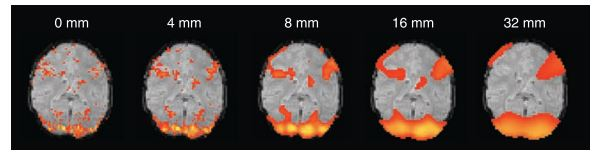
\includegraphics[width=.8\textwidth]{figures/aBackground/smooth}  
	\caption{Illustration showing the impact of using different distribution width on the activated areas. An increase in width results in greater areas of activation smearing together and the removal of smaller.\cite{Poldrack2011}}
	\label{fig:back:smooth} 
\end{figure}  


